\documentclass[portfolio.tex]{subfiles}
\begin{document}
	\Chapter{Week 5}{Model View Design Patterns}
		\section{Weekly Content}
			\subsection{Introduction}
				The new concept for this week was UI design patterns. Two of the most well known are MVC and MVVM. This is relevant theoretical knowledge since Vue is an example of MVVM. If we are better able to understand this design pattern, then we can intern better understand Vue and its capabilities.

			\subsection{MVC}
				\splitpage{
					\centering
					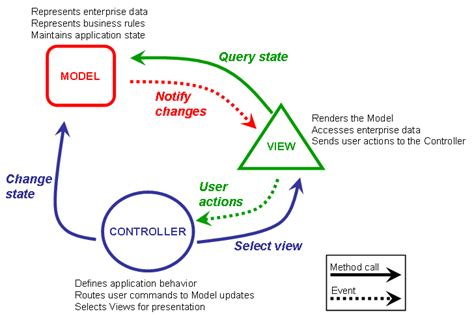
\includegraphics[width=\textwidth]{mvc.png}\\
					 \autocite{mvc-image}
				}{
					\textbf{M}odel \textbf{V}iew \textbf{C}ontroller was the original Model-View design. This model looked to solve how to structure large front end codebases, and separate areas of concern. As the name suggests it was made of up three components, a model, a view and a controller.
				}


				\subsubsection{Controller}
					The controller handles all user interactions or events. When a button is clicked, the controller will decide what to do and modify the model accordingly. The controller is also in charge of which view to present to the user. This way many different views could be used depending on the situation.

				\subsubsection{Model}
					This contains the data that will be loaded into the webpage.  This is the component that will get information from a back-end or database, and is in charge of the applications state.

				\subsubsection{View}
					What the user sees. Using the observer pattern, the view is notified when a change occurs to the model, and then the view will fetch the new data.

					\autocite{mv-design}

			\subsection{MVVM}
				\textbf{M}odel \textbf{V}iew \textbf{V}iew \textbf{M}odel builds upon MVC. The main benefit of this is being able to reuse the business logic for multiple view-controllers, making the controller more UI focussed.


				\begin{center}
					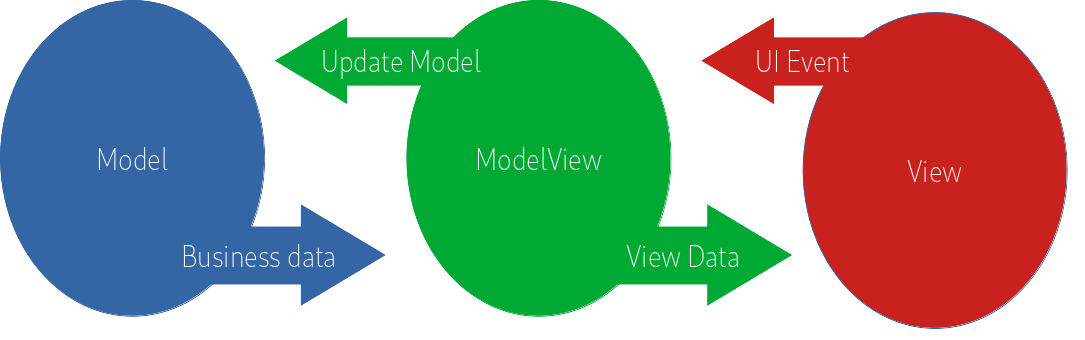
\includegraphics[width=0.8\linewidth]{mvvm.png}
				\end{center}

				\subsubsection{View}
					MVVM considers the view and the controller to be tightly coupled. This means that view handles both the displaying of information, as well as user inputs and events. The view can also pull data from the View Model and trigger methods within the view model based on user input.

				\subsubsection{View-Model}
					The new component added when compared to MVC. It works between view and model. It handles all the logic and state within the application. View-model is unaware of view. Any updates within the view-model will be announced to subscribers, and then the subscribers can grab the update.

				\subsubsection{Model}
					This is very similar to the model in MVC. Model is unaware of view or view-model. It simply supplies the data to the application and modifies this data on request.\\

				\autocite{mv-design}

		\section{Practical Tasks}
			\subsection{Introduction}
				Building on last weeks theoretical introduction to Vue concepts, this week we implement them within our own project. Practicing these concepts, and seeing them in action, will help our understanding of the theoretical side.\\


			\subsection{Task 1}
				Components are ways to reuse pieces of code. Both presentation code and logic can be reused within elements that perform similar tasks. This allows less repetition of code and the ability to build applications much quicker.\\

				The syntax for defining a component is:\\
				\label{global-registration}
				\begin{lstlisting}
Vue.component('component-name', {
	template: '<h1>This is a component</h1>'
})
				\end{lstlisting}

				\vspace{0.5cm} \noindent Then to use this component simply use the tag in the html like so:\\

				\begin{center}
					$<$component-name /$>$
				\end{center}

				\vspace{0.5cm} \noindent This will output the header, "This is a component", into the DOM.\\

				Within my project, I have already used a few components, to encapsulate views, or to group re-usable code together. The most reused so far would be ImageCard, which is reused many times within Image Gallery. In the screenshot below, each picture is a separate ImageCard component which handles the click, hover and data display.

				\begin{center}
					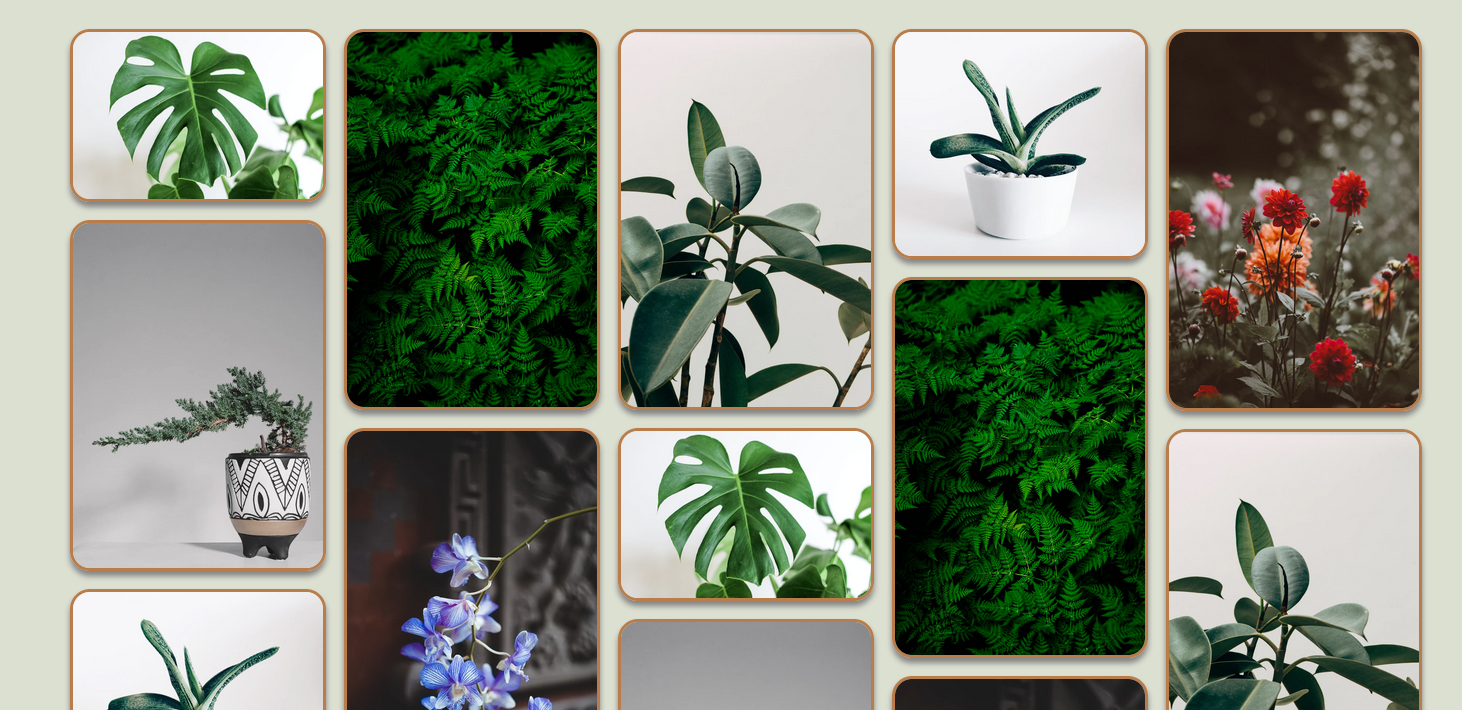
\includegraphics[width=0.8\linewidth]{image-card-example.png}
				\end{center}


				\subsubsection{Source Code}
					\noindent For a full list of components I have created see:  \\
					\seqsplit{https://github.com/BrandonMurch/SIT120/tree/main/Assignment\%201/proof-of-concept/src/components.}

			\subsection{Task 2}
				I have explored Vue and implemented concepts so far in my project, as well as discussed them previously in this report. See:
				\\ \seqsplit{https://github.com/BrandonMurch/SIT120/tree/main/Assignment\%201/proof-of-concept/src/}.

			\subsection{Task 3}
				To handle user input the \textbf{v-on} (or the shorthand \textbf{@}) keywords can be used. This can be used with many native events such as \textbf{click}. It can also be used for custom events. I have described such events here: \ref{custom-events}. \\

				These events can either call methods in the methods object or they can modify properties within the data object directly. \\

				As with previous tasks, I have also used event handling throughout my project. A specific example is watching for clicks on buttons using @click within the PopUp component. Where clicking the \\

				\subsubsection{Source Code}
				\seqsplit{https://github.com/BrandonMurch/SIT120/blob/main/Assignment\%201/proof-of-concept/src/components/PopUp.vue}


			\subsection{Task 4}
				\label{task4}
				\subsubsection{Component Registration}
					With Vue, components can be registered globally (\ref{global-registration}), or locally. To register a component locally, just store the component in a local variable like so:\\

					\begin{lstlisting}
const component = { .... }
					\end{lstlisting}

					\bigbreak

					Alternatively Vue components can be placed in their own \textbf{.vue} file. Their declaration is handled implicitly, and the file can contain three tags [template, script and style] which contain the relevant HTML, JavaScript and CSS respectively.\\

					\noindent For a more in-depth description of Vue component registration, see \ref{vue-component-registration}

				\subsubsection{Props}
					If we just used components with the same values every time, they wouldn't be very reusable or useful. By defining options that can be passed into the component as "props", components become much more useful and versatile.

					 Using the \textbf{v-bind} keyword we are able to pass in this data. If the component accepted a prop \textbf{message}, then to pass in a message, use v-bind:\\

					\begin{lstlisting}
<component-name v-bind:message="This is a message!" />
					\end{lstlisting}

					The shorthand for v-bind would be simply \textbf{:}message="..."\\

				\subsubsection{Custom Events and Slots}
					See \ref{custom-events} for custom events and \ref{slots} for slots.

				\subsubsection{Dynamic and Async Components}
					Dynamic components allow us to select which component to render dynamically. To do this, use the following syntax:\\

					\begin{lstlisting}
<component v-bind:is="myDynamicallySelectedComponent">
</component>
					\end{lstlisting}

					\vspace{0.5cm}
					Putting elements inside the $<$keep-alive$>$ element, as the name suggests will keep the component alive. That is, the component will not be destroyed. This helps with loading times on elements that are frequently switched between, or whose information won't change. \\

					Components can be rendered asynchronously. An example of this would be when the component renders only after information is received from the backend server. These components can even load other components while they are loading, or if there is an error.

					There are a few ways to accomplish this within Vue. The first is to return the component as a promise resolve:\\

					\begin{lstlisting}
Vue.component('async-webpack-example', function (resolve) {
	require(['./my-async-component'], resolve)
})
					\end{lstlisting}
					\autocite{vue-async}\\

					\bigbreak

					Another is dynamically importing the component:\\

					\begin{lstlisting}
Vue.component(
	'async-webpack-example',
	() => import('./my-async-component')
)
					\end{lstlisting}
					\autocite{vue-async}\\

					\bigbreak
					Finally Vue can also handle the loading, errors, delay and timeout of these async components using the following:\\

					\begin{lstlisting}
const AsyncComponent = () => ({
	// The component to load (should be a Promise)
	component: import('./MyComponent.vue'),
	// A component to use while the async component is loading
	loading: LoadingComponent,
	// A component to use if the load fails
	error: ErrorComponent,
	// Delay before showing the loading component. Default: 200ms.
	delay: 200,
	// The error component will be displayed if a timeout is
	// provided and exceeded. Default: Infinity.
	timeout: 3000
})
					\end{lstlisting}
					\autocite{vue-async}

				\subsubsection{Handling Edge Cases}
					There are cases when the strict nature of Vue needs to be broken, giving more access to the developer. These cases are very rare, and have serious drawbacks, so they should not be used lightly.\\

					Within Vue, any subcomponent can reference the root component with \$root. This is particularly handy when using the root as a store. A better alternative is to use Vuex, which is discussed here \ref{vuex}.\\



					Similarly, \$parent can be used to access the parent component. This is generally reserved for very special cases and most of the time can simply be a mask for poor design. Instead use props, events and two-way binding.\\

					\vspace{0.5cm}
					\hspace{-1.6cm}
					\splitpage{
						\centering
						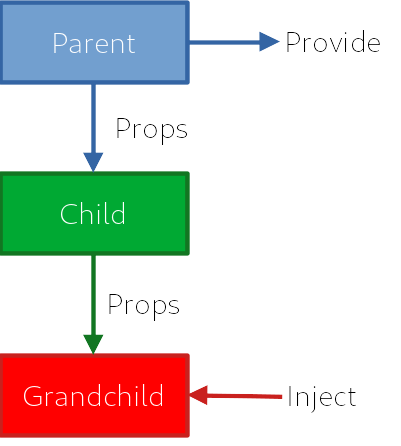
\includegraphics[width=0.8\linewidth]{injection.png}
					}{
						A way to avoid prop drilling (passing information down multiple layers of components) is to use the provide and inject options. In the parent use the option provide to supply data or method. Then within the child using inject, the child will be able to access the provided data/method. The downside is that this tightly couples the component to the current structural design. Any reshuffling of structure will lead to bugs that might not be immediately obvious. . \\
					}

					\vspace{0.5cm}

					Event listeners can be programatically managed within Vue. There are three options: \$on to add an event listener, \$once to add an event listener that only listens for the first event and \$off to remove an event listener.\\

					The \$forceUpdate method can be called to manually force an update on the component. This is primarily if there is external data that causes an update.\\
		\section{Project}
			\subsection{What I accomplished this week}
				I decided against working on my web app this week until I receive the feedback from my proposal to ensure I am  working in the right direction. I will use this time to get ahead on other courses so that I can focus on my application next week.

			\subsection{What I would like to accomplish next week}
				This week I would like to incorporate Vue-Router into my program, and start creating the other parts of the website (My Plants, and Learn). The main reusable components I will need for this are lists to display cards for comments, articles, etc. Another important part will be to create the interface for adjusting plant settings. I suspect this all will take 4 hours.

\pagebreak
\end{document}